\documentclass[xcolor=dvipsnames]{beamer}\usepackage[]{graphicx}\usepackage[]{color}
%% maxwidth is the original width if it is less than linewidth
%% otherwise use linewidth (to make sure the graphics do not exceed the margin)
\makeatletter
\def\maxwidth{ %
  \ifdim\Gin@nat@width>\linewidth
    \linewidth
  \else
    \Gin@nat@width
  \fi
}
\makeatother

\definecolor{fgcolor}{rgb}{0.345, 0.345, 0.345}
\newcommand{\hlnum}[1]{\textcolor[rgb]{0.686,0.059,0.569}{#1}}%
\newcommand{\hlstr}[1]{\textcolor[rgb]{0.192,0.494,0.8}{#1}}%
\newcommand{\hlcom}[1]{\textcolor[rgb]{0.678,0.584,0.686}{\textit{#1}}}%
\newcommand{\hlopt}[1]{\textcolor[rgb]{0,0,0}{#1}}%
\newcommand{\hlstd}[1]{\textcolor[rgb]{0.345,0.345,0.345}{#1}}%
\newcommand{\hlkwa}[1]{\textcolor[rgb]{0.161,0.373,0.58}{\textbf{#1}}}%
\newcommand{\hlkwb}[1]{\textcolor[rgb]{0.69,0.353,0.396}{#1}}%
\newcommand{\hlkwc}[1]{\textcolor[rgb]{0.333,0.667,0.333}{#1}}%
\newcommand{\hlkwd}[1]{\textcolor[rgb]{0.737,0.353,0.396}{\textbf{#1}}}%

\usepackage{framed}
\makeatletter
\newenvironment{kframe}{%
 \def\at@end@of@kframe{}%
 \ifinner\ifhmode%
  \def\at@end@of@kframe{\end{minipage}}%
  \begin{minipage}{\columnwidth}%
 \fi\fi%
 \def\FrameCommand##1{\hskip\@totalleftmargin \hskip-\fboxsep
 \colorbox{shadecolor}{##1}\hskip-\fboxsep
     % There is no \\@totalrightmargin, so:
     \hskip-\linewidth \hskip-\@totalleftmargin \hskip\columnwidth}%
 \MakeFramed {\advance\hsize-\width
   \@totalleftmargin\z@ \linewidth\hsize
   \@setminipage}}%
 {\par\unskip\endMakeFramed%
 \at@end@of@kframe}
\makeatother

\definecolor{shadecolor}{rgb}{.97, .97, .97}
\definecolor{messagecolor}{rgb}{0, 0, 0}
\definecolor{warningcolor}{rgb}{1, 0, 1}
\definecolor{errorcolor}{rgb}{1, 0, 0}
\newenvironment{knitrout}{}{} % an empty environment to be redefined in TeX

\usepackage{alltt}
% sets the beamer them and color
\usetheme{CambridgeUS}
\usecolortheme{seahorse}
% turns off navigation bar
\beamertemplatenavigationsymbolsempty
% allows inclusion of graphics and makes equations larger
\usepackage{graphicx}
\newcommand*{\Scale}[2][4]{\scalebox{#1}{\ensuremath{#2}}}%
% uses my custom bibliography style
\usepackage[authoryear,round]{natbib}
  \bibliographystyle{c:/aaaWork/zGnrlLatex/afs}
  \bibpunct{(}{)}{;}{a}{}{,}
% allows saving and starting a counter across slides
\newcounter{resEnumi}
\newcommand{\saveResEnumi}{\setcounter{resEnumi}{\theenumi}}
\newcommand{\setResEnumi}{\setcounter{enumi}{\theresEnumi}}
% reduce footnote size
\setbeamerfont{footnote}{size=\tiny}
% allows coloring of tables
\usepackage{colortbl}
\definecolor{light-gray}{gray}{0.95}
% for color in equations
\makeatletter
\def\mathcolor#1#{\@mathcolor{#1}}
\def\@mathcolor#1#2#3{%
  \protect\leavevmode
  \begingroup
    \color#1{#2}#3%
  \endgroup
}
\makeatother





%###############################################################################
%###############################################################################
% Start the document.
\IfFileExists{upquote.sty}{\usepackage{upquote}}{}
\begin{document}

% Make a title slide
\title[Critical Time from Modified VBGF]{Modified von Bertalanffy Growth Function to Directly Estimate the Age at a Critical Length}
\author[Ogle \& Isermann]{Dr. Derek H. Ogle \inst{1} and Dr. Daniel A. Isermann \inst{2}}
\institute[]{\normalsize \inst{1}Mathematical Sciences \& Natural Resources, Northland College \and %
\inst{2}U. S. Geological Survey, Wisconsin Cooperative Fishery Research Unit,\\ College of Natural Resources, University of Wisconsin-Stevens Point}
\date[WI AFS 2016]{ \\[2\baselineskip] Wisconsin AFS -- LaCrosse, WI -- 28 February 2016}
\maketitle

% Setup a TOC that will be repeated at each section
\AtBeginSection[] {
\begin{frame}[t]
\frametitle{}
\tableofcontents[currentsection]
\end{frame}
}



%###############################################################################
%###############################################################################
\section{Critical Time Concept}

\begin{frame}[fragile, t]
\frametitle{Definitions}
\begin{itemize}
  \item Critical points in a fish's life are often defined.
  \begin{itemize}
    \item e.g., age at maturity, recruitment, a length defined by a regulation.
  \end{itemize}
\end{itemize}
\pause
\smallskip
\begin{minipage}[t]{0.6\textwidth}
  \begin{itemize}
    \item $L_{r}$
    \begin{itemize}
      \item Length at critical point.
      \item Defined by scientist.
    \end{itemize}
  \end{itemize}
\end{minipage}%
\hspace*{-2cm}
\begin{minipage}[t]{0.7\textwidth}
\begin{knitrout}\footnotesize
\definecolor{shadecolor}{rgb}{0.969, 0.969, 0.969}\color{fgcolor}

{\centering 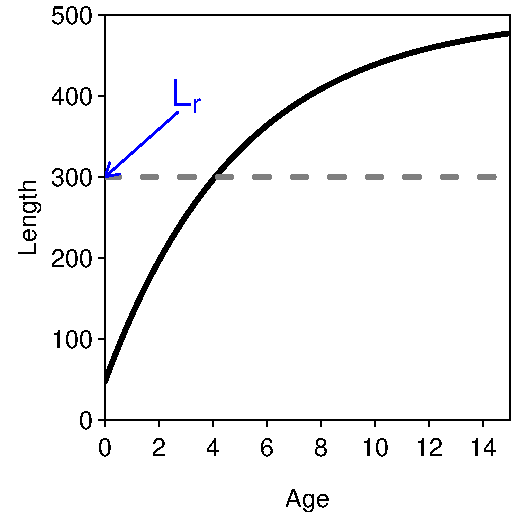
\includegraphics[width=.6\linewidth]{Figs/defn1-1} 

}



\end{knitrout}
\end{minipage}%
\end{frame}


\begin{frame}[fragile, t]
\frametitle{Definitions}
\begin{itemize}
  \item Critical points in a fish's life are often defined.
  \begin{itemize}
    \item e.g., age at maturity, recruitment, a length defined by a regulation.
  \end{itemize}
\end{itemize}
\smallskip
\begin{minipage}[t]{0.6\textwidth}
  \begin{itemize}
    \item $L_{r}$
    \begin{itemize}
      \item Length at critical point.
      \item Defined by scientist.
    \end{itemize}
    \smallskip
    \item $t_{r}$
    \begin{itemize}
      \item Age (time) at the critical point.
      \item To be estimated.
    \end{itemize}
  \end{itemize}
\end{minipage}%
\hspace*{-2cm}
\begin{minipage}[t]{0.7\textwidth}
\begin{knitrout}\footnotesize
\definecolor{shadecolor}{rgb}{0.969, 0.969, 0.969}\color{fgcolor}

{\centering 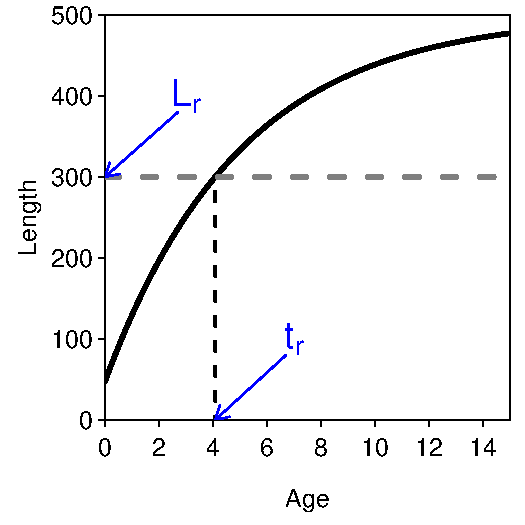
\includegraphics[width=.6\linewidth]{Figs/defn2-1} 

}



\end{knitrout}
\end{minipage}%
\end{frame}


\begin{frame}[fragile, t]
\frametitle{Importance}
\begin{itemize}
  \item Undestanding $t_{r}$ is important.
  \pause
  \bigskip
\end{itemize}

\hspace*{-1cm}
\begin{minipage}{0.7\textwidth}
\begin{knitrout}\footnotesize
\definecolor{shadecolor}{rgb}{0.969, 0.969, 0.969}\color{fgcolor}

{\centering 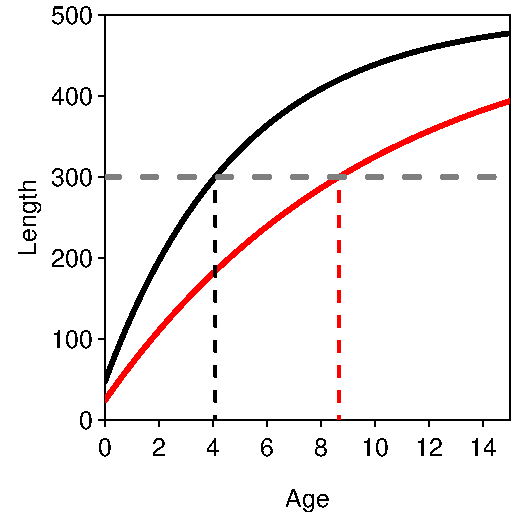
\includegraphics[width=.5\linewidth]{Figs/unnamed-chunk-1-1} 

}



\end{knitrout}
\end{minipage}%
\pause
\hspace*{-3cm}
\begin{minipage}{0.7\textwidth}
\begin{knitrout}\footnotesize
\definecolor{shadecolor}{rgb}{0.969, 0.969, 0.969}\color{fgcolor}

{\centering 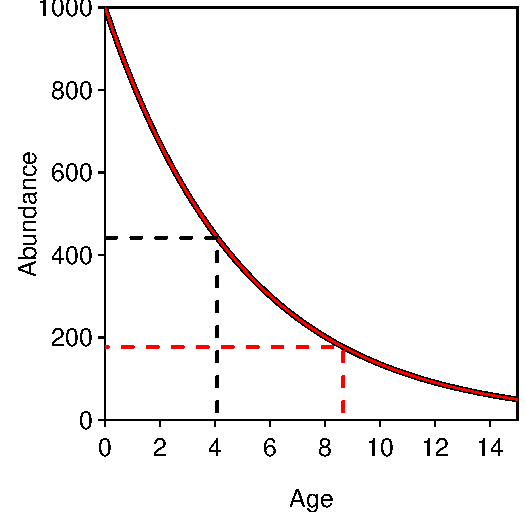
\includegraphics[width=.5\linewidth]{Figs/unnamed-chunk-2-1} 

}



\end{knitrout}
\end{minipage}
\end{frame}


\begin{frame}[fragile, t]
\frametitle{Importance}
\begin{itemize}
  \item Foundational value in \textit{yield-per-recruit} and \textit{dynamic pool} models.
  \begin{itemize}
    \item Commonly used to examine the impact of length regulations.
  \end{itemize}
\end{itemize}
\pause
\begin{center}
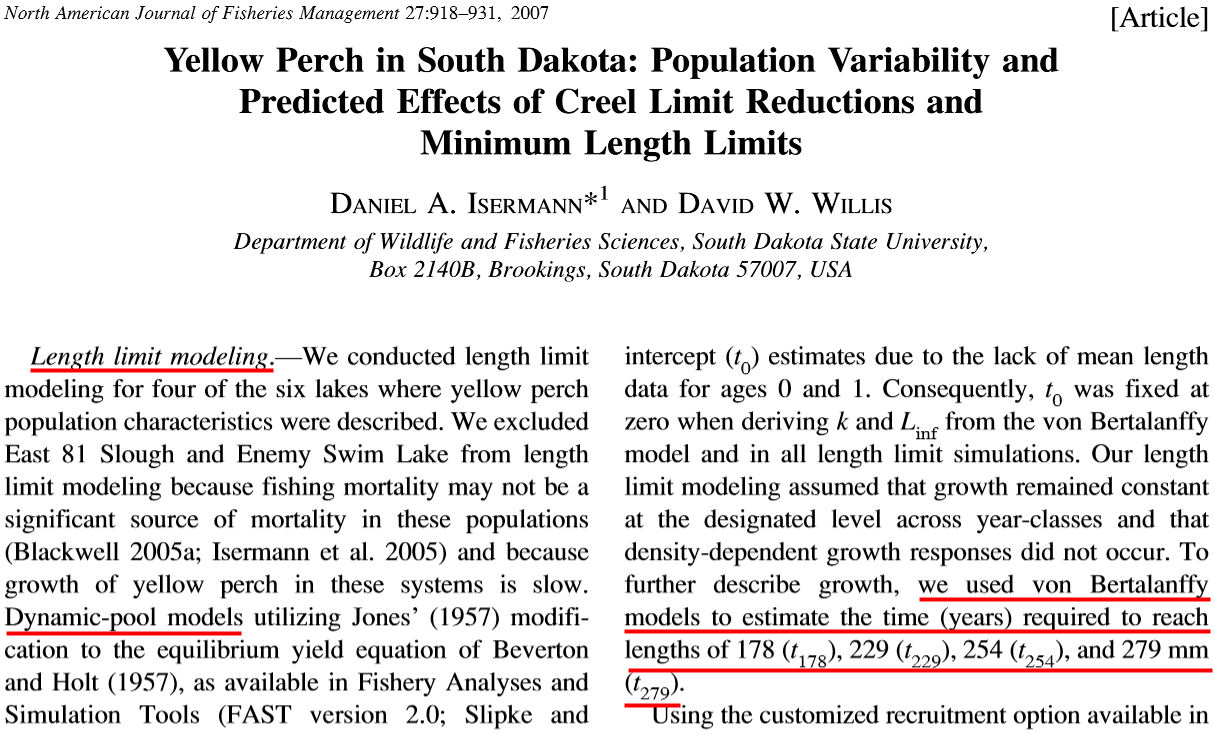
\includegraphics[width=3.7in]{Figs/Isermann-etal-2007.jpg}
\end{center}
\end{frame}


\begin{frame}[fragile, t]
\frametitle{Importance}
\begin{itemize}
  \item Foundational value in \textit{yield-per-recruit} and \textit{dynamic pool} models.
  \begin{itemize}
    \item Commonly used to examine impact of length regulations.
  \end{itemize}
\end{itemize}

\smallskip

\begin{center}

\includegraphics[width=4.7in]{Figs/tr-examples.jpg}
\end{center}
\end{frame}


%###############################################################################
%###############################################################################
\section{$t_{r}$ Often Estimated by Inverting the VBGF}

\begin{frame}[fragile, t]
\frametitle{von Bertalanffy Growth Function Review}

\[\Scale[1.5]{ L_{t} = L_{\infty}\left(1-e^{-K(t-t_{0})}\right) }\]

\bigskip
\begin{knitrout}\footnotesize
\definecolor{shadecolor}{rgb}{0.969, 0.969, 0.969}\color{fgcolor}

{\centering 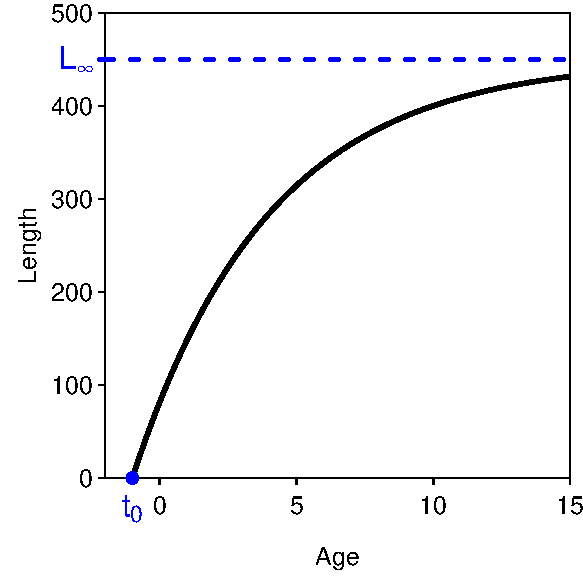
\includegraphics[width=.47\linewidth]{Figs/unnamed-chunk-3-1} 

}



\end{knitrout}
\end{frame}


\begin{frame}[fragile, t]
\frametitle{Inverting the VBGF}

\[\Scale[1.5]{ L_{t} = L_{\infty}\left(1-e^{-K(t-t_{0})}\right) }\]

\bigskip
\begin{itemize}
  \item The \textit{inverse VBGF} is found by algebraically solving the VBGF for $t$.
  \pause
  \bigskip

\[\Scale[1.5]{ t = \frac{log_{e}\left(1-\frac{L_{t}}{L_{\infty}}\right)}{-K} + t_{0} }\]

  \pause
  \bigskip
  \item Then set $L_{t}$ to the chosen $L_{r}$ so that $t$ will be $t_{r}$.
\end{itemize}
\end{frame}


\begin{frame}[fragile, t]
\frametitle{Computing $t_{r}$ from Inverse VBGF}
\[\Scale[1.5]{ t = \frac{log_{e}\left(1-\frac{L_{t}}{L_{\infty}}\right)}{-K} + t_{0} }\]
  \smallskip
\begin{itemize}
  \item Suppose that $L_{\infty}$=450, $K$=0.2, and $t_{0}$=-1.
  \item Suppose that the critical length of interest is $L_{r}$=300.
  \pause
  \smallskip
\[\Scale[1.5]{ t = \frac{log_{e}\left(1-\frac{300}{450}\right)}{-0.2} + -1 = 4.5}\]
  \pause
  \smallskip
  \item Thus, the estimated mean time to reach 300 mm is 4.5 years.
\end{itemize}
\end{frame}


\begin{frame}[fragile, t]
\frametitle{Computing $t_{r}$ from Inverse VBGF}
\begin{center}
{\LARGE That was easy}
\end{center}
\pause
\vspace{0.25in}
\begin{itemize}
  \item \textcolor{red}{BUT} ... how do you compute confidence intervals for $t_{r}$?
  \pause
  \begin{itemize}
    \item Could use bootstrap, delta method, or error propagation.
    \item Could \emph{try} to fit inverse function and predict $t_{r}$ at $L_{r}$.
  \end{itemize}
  \pause
  \bigskip
  \item \textcolor{red}{BUT} ... how do you compare $t_{r}$ between groups?
\end{itemize}
\pause
\vspace{0.5in}
\begin{center}
{\LARGE We need a better method!}
\end{center}
\end{frame}



%###############################################################################
%###############################################################################
\section{Reparamereterize the VBGF to Estimate $t_{r}$}


\begin{frame}[fragile, t]
\frametitle{Revist VBGF}
\begin{itemize}
\item The typical VBGF ...

\[\Scale[1.5]{ L_{t} = L_{\infty}\left(1-e^{-K(t-t_{0})}\right) }\]

\bigskip
\item ... may be rewritten as ...

\[\Scale[1.5]{ L_{t} = \mathcolor{blue}{0} + (L_{\infty}-\mathcolor{blue}{0})\left(1-e^{-K(t-t_{0})}\right) }\]
\end{itemize}
\end{frame}


\begin{frame}
\frametitle{Revist VBGF}
\vspace{-14pt}
\[\Scale[1.5]{ L_{t} = \mathcolor{blue}{0} + (L_{\infty}-\mathcolor{blue}{0})\left(1-e^{-K(t-t_{0})}\right) }\]
\vspace{14pt}

\begin{knitrout}\footnotesize
\definecolor{shadecolor}{rgb}{0.969, 0.969, 0.969}\color{fgcolor}

{\centering 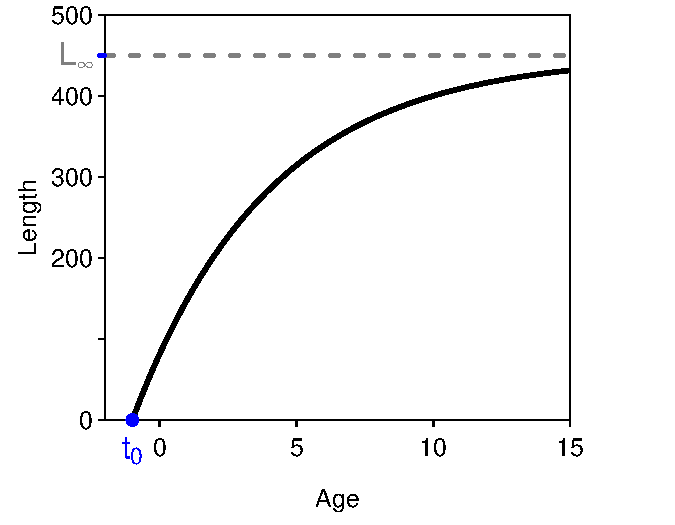
\includegraphics[width=.5\linewidth]{Figs/redefineB-1} 

}



\end{knitrout}

\begin{itemize}
  \item The typical VBGF estimates $t_{0}$ for $L=0$.
\end{itemize}
\end{frame}


\begin{frame}[fragile, t]
\frametitle{Revist VBGF}
\begin{itemize}
\item The original VBGF (from von Bertalanffy) ...

\[\Scale[1.5]{ L_{t} = L_{0} + (L_{\infty}-L_{0})\left(1-e^{-Kt}\right) }\]

\bigskip
\item ... can be rewritten ...

\[\Scale[1.5]{ L_{t} = L_{0} + (L_{\infty}-L_{0})\left(1-e^{-K(t-\mathcolor{red}{0})}\right) }\]
\end{itemize}
\end{frame}


\begin{frame}
\frametitle{Revist VBGF}
\vspace{-14pt}
\[\Scale[1.5]{ L_{t} = L_{0} + (L_{\infty}-L_{0})\left(1-e^{-K(t-\mathcolor{red}{0})}\right) }\]
\vspace{14pt}
\begin{knitrout}\footnotesize
\definecolor{shadecolor}{rgb}{0.969, 0.969, 0.969}\color{fgcolor}

{\centering 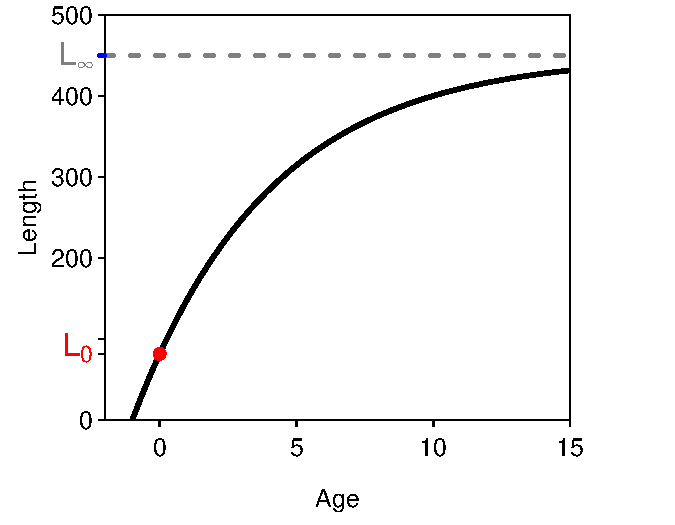
\includegraphics[width=.5\linewidth]{Figs/redefineC-1} 

}



\end{knitrout}

\begin{itemize}
\item The original VBGF estimates $L_{0}$ for $t=0$.
\end{itemize}
\end{frame}


\begin{frame}
\frametitle{Revist VBGF}
\vspace{-12pt}
\begin{itemize}
\item These VBGFs simply define different points on the same line.

\[\Scale[1.3]{ L_{t} = \mathcolor{blue}{0} + (L_{\infty}-\mathcolor{blue}{0})\left(1-e^{-K(t-t_{0})}\right) }\]
\[\Scale[1.3]{ L_{t} = L_{0} + (L_{\infty}-L_{0})\left(1-e^{-K(t-\mathcolor{red}{0})}\right) }\]

\pause
\smallskip
\item Can a more useful point on the line be defined?
  \pause
  \begin{itemize}
    \item A more general VBGF is

\[\Scale[1.3]{ L_{t} = \mathcolor{red}{L_{r}} + (L_{\infty}-\mathcolor{red}{L_{r}})\left(1-e^{-K(t-\mathcolor{red}{t_{r}})}\right) }\]

    \pause
    \item where ...
      \begin{itemize}
        \item Typical VBGF sets $L_{r}=0$ and estimates $t_{r}=t_{0}$.
        \item Original VBGF sets $t_{r}=0$ and estimates $L_{r}=L_{0}$.
      \end{itemize}
    \pause
    \smallskip
    \item \textbf{However, we can also set $L_{r}$ to a critical length and estimate $t_{r}$}.
  \end{itemize}
\end{itemize}
\end{frame}



%###############################################################################
%###############################################################################
\section{An Example with Lake Michigan Lake Whitefish}




\begin{frame}[fragile, t]
\frametitle{Example with Lake Michigan Lake Whitefish}
\begin{itemize}
  \item Data from Belnap (2014).\footnotemark
  \footnotetext[1]{Belnap, M.J. 2014. Stock Characteristics of Lake Whitefish in Lake Michigan. M.Sc. Thesis, Univ. Wis. - Stevens Point.}
  \begin{itemize}
    \item Fish from commercial trapnets in six management zones.
    \item Measured total length (TL; mm).
    \item Estimated age (yrs) from otolith thin sections.
    \item Interested in $t_{480}$ (480 mm is length at full vulnerability to harvest).
  \end{itemize}
  \pause
  \bigskip
  \item Fit traditional and modified VBGF to fish from Big Bay de Noc.
  \begin{itemize}
    \item Compared parameter estimates and predicted mean lengths-at-age.
  \end{itemize}
  \pause
  \smallskip
  \item Fit modified VBGF to fish from Big Bay de Noc and Green Bay to illustrate $t_{r}$ comparison (following methods in Ogle (2016)\footnotemark).
  \footnotetext[2]{Ogle, D.H. 2016.  Introductory Fisheries Analyses with R.  CRC Press, Boca Raton, FL.}
\end{itemize}
\end{frame}


\begin{frame}[fragile, t]
\frametitle{Comparison of VBGF Results}
\begin{columns}
\begin{column}{0.5\textwidth}
\textbf{Traditional VBGF}
% latex table generated in R 3.2.3 by xtable 1.8-0 package
% Sun Jan 31 18:26:25 2016
\begin{table}[ht]
\centering
\begin{tabular}{rrrr}
  \hline
 & Estimate & LCI & UCI \\ 
  \hline
$L_{\infty}$ & 549.51 & 541.56 & 560.99 \\ 
  $K$ & 0.29 & 0.19 & 0.39 \\ 
  $t_{0}$ & 2.70 & -0.32 & 4.32 \\ 
  $t_{480}$ & 9.88 & - & - \\ 
   \hline
\end{tabular}
\end{table}

\end{column}
\begin{column}{0.5\textwidth}
\end{column}
\end{columns}
\end{frame}


\begin{frame}[fragile, t]
\frametitle{Comparison of VBGF Results}
\begin{columns}
\begin{column}{0.5\textwidth}
\textbf{Traditional VBGF}
% latex table generated in R 3.2.3 by xtable 1.8-0 package
% Sun Jan 31 18:26:25 2016
\begin{table}[ht]
\centering
\begin{tabular}{rrrr}
  \hline
 & Estimate & LCI & UCI \\ 
  \hline
$L_{\infty}$ & 549.51 & 541.56 & 560.99 \\ 
  $K$ & 0.29 & 0.19 & 0.39 \\ 
  $t_{0}$ & 2.70 & -0.32 & 4.32 \\ 
  $t_{480}$ & 9.88 & - & - \\ 
   \hline
\end{tabular}
\end{table}

\end{column}
\begin{column}{0.5\textwidth}
\textbf{Modified VBGF}
% latex table generated in R 3.2.3 by xtable 1.8-0 package
% Sun Jan 31 18:26:25 2016
\begin{table}[ht]
\centering
\begin{tabular}{rrrr}
  \hline
 & Estimate & LCI & UCI \\ 
  \hline
$L_{\infty}$ & 549.51 & 541.56 & 560.99 \\ 
  $K$ & 0.29 & 0.19 & 0.39 \\ 
  $t_{0}$ & - & - & - \\ 
  $t_{480}$ & 9.88 & 9.43 & 10.28 \\ 
   \hline
\end{tabular}
\end{table}

\end{column}
\end{columns}
\end{frame}


\begin{frame}[fragile, t]
\frametitle{Comparison of VBGF Results}
\begin{columns}
\begin{column}{0.5\textwidth}
\textbf{Traditional VBGF}
% latex table generated in R 3.2.3 by xtable 1.8-0 package
% Sun Jan 31 18:26:25 2016
\begin{table}[ht]
\centering
\begin{tabular}{rrrr}
  \hline
 & Estimate & LCI & UCI \\ 
  \hline
$L_{\infty}$ & 549.51 & 541.56 & 560.99 \\ 
  $K$ & 0.29 & 0.19 & 0.39 \\ 
  $t_{0}$ & 2.70 & -0.32 & 4.32 \\ 
  $t_{480}$ & 9.88 & - & - \\ 
   \hline
\end{tabular}
\end{table}

\smallskip
% latex table generated in R 3.2.3 by xtable 1.8-0 package
% Sun Jan 31 18:26:25 2016
\begin{table}[ht]
\centering
\begin{tabular}{rr}
  \hline
Age & Pred Len \\ 
  \hline
8.00 & 429.97 \\ 
  15.00 & 533.56 \\ 
  25.00 & 548.61 \\ 
  9.88 & 480.00 \\ 
   \hline
\end{tabular}
\end{table}

\end{column}
\begin{column}{0.5\textwidth}
\textbf{Modified VBGF}
% latex table generated in R 3.2.3 by xtable 1.8-0 package
% Sun Jan 31 18:26:25 2016
\begin{table}[ht]
\centering
\begin{tabular}{rrrr}
  \hline
 & Estimate & LCI & UCI \\ 
  \hline
$L_{\infty}$ & 549.51 & 541.56 & 560.99 \\ 
  $K$ & 0.29 & 0.19 & 0.39 \\ 
  $t_{0}$ & - & - & - \\ 
  $t_{480}$ & 9.88 & 9.43 & 10.28 \\ 
   \hline
\end{tabular}
\end{table}

\smallskip
% latex table generated in R 3.2.3 by xtable 1.8-0 package
% Sun Jan 31 18:26:25 2016
\begin{table}[ht]
\centering
\begin{tabular}{rr}
  \hline
Age & Pred Len \\ 
  \hline
8.00 & 429.97 \\ 
  15.00 & 533.56 \\ 
  25.00 & 548.61 \\ 
  9.88 & 480.00 \\ 
   \hline
\end{tabular}
\end{table}

\end{column}
\end{columns}
\end{frame}




\begin{frame}[fragile, t]
\frametitle{Comparing $t_{r}$ Between Groups}
\begin{itemize}
  \item Fit all (8) models where all, two, one, or no parameters differ between the two locations (Big Bay de Noc and Green Bay).
\end{itemize}
\pause
\bigskip
% latex table generated in R 3.2.3 by xtable 1.8-0 package
% Sun Jan 31 18:26:25 2016
\begin{table}[ht]
\centering
\begin{tabular}{lrrrr}
  \hline
Model & Params & AICc & $\Delta$AICc & Weight \\ 
  \rowcolor{light-gray} \hline
$L_{\infty}$, $t_{480}$ & 6 & 3203.3 & 0.00 & 0.38 \\ 
   \rowcolor{light-gray}$K$, $t_{480}$ & 6 & 3203.5 & 0.19 & 0.34 \\ 
   \rowcolor{light-gray}$L_{\infty}$, $K$, $t_{480}$ & 7 & 3204.7 & 1.40 & 0.19 \\ 
   \rowcolor{light-gray}$t_{480}$ & 5 & 3206.2 & 2.90 & 0.09 \\ 
  $L_{\infty}$ & 5 & 3221.2 & 17.91 & 0.00 \\ 
  $K$ & 5 & 3222.5 & 19.14 & 0.00 \\ 
  $L_{\infty}$, $K$ & 6 & 3223.3 & 19.97 & 0.00 \\ 
  None & 4 & 3230.0 & 26.68 & 0.00 \\ 
   \hline
\end{tabular}
\end{table}

\end{frame}


\begin{frame}[fragile, t]
\frametitle{Comparing $t_{r}$ Between Groups}
\begin{columns}
\begin{column}{0.5\textwidth}
\textbf{Big Bay de Noc}
% latex table generated in R 3.2.3 by xtable 1.8-0 package
% Sun Jan 31 18:26:25 2016
\begin{table}[ht]
\centering
\begin{tabular}{rrrr}
  \hline
 & Estimate & LCI & UCI \\ 
  \hline
$L_{\infty}$ & 549.51 & 541.79 & 560.50 \\ 
  $K$ & 0.29 & 0.20 & 0.38 \\ 
   \rowcolor{light-gray}$t_{480}$ & 9.88 & 9.44 & 10.27 \\ 
   \hline
\end{tabular}
\end{table}

\end{column}
\begin{column}{0.5\textwidth}
\textbf{Green Bay}
% latex table generated in R 3.2.3 by xtable 1.8-0 package
% Sun Jan 31 18:26:25 2016
\begin{table}[ht]
\centering
\begin{tabular}{rrrr}
  \hline
 & Estimate & LCI & UCI \\ 
  \hline
$L_{\infty}$ & 555.91 & 546.84 & 571.16 \\ 
  $K$ & 0.39 & 0.18 & 1.23 \\ 
   \rowcolor{light-gray}$t_{480}$ & 7.56 & 6.20 & 8.48 \\ 
   \hline
\end{tabular}
\end{table}

\end{column}
\end{columns}
\end{frame}


\begin{frame}[fragile, t]
\frametitle{Comparing $t_{r}$ Between Groups}
\begin{columns}
\begin{column}{0.5\textwidth}
\textbf{Big Bay de Noc}
% latex table generated in R 3.2.3 by xtable 1.8-0 package
% Sun Jan 31 18:26:25 2016
\begin{table}[ht]
\centering
\begin{tabular}{rrrr}
  \hline
 & Estimate & LCI & UCI \\ 
  \rowcolor{light-gray} \hline
$t_{480}$ & 9.88 & 9.44 & 10.27 \\ 
   \hline
\end{tabular}
\end{table}

\end{column}
\begin{column}{0.5\textwidth}
\textbf{Green Bay}
% latex table generated in R 3.2.3 by xtable 1.8-0 package
% Sun Jan 31 18:26:26 2016
\begin{table}[ht]
\centering
\begin{tabular}{rrrr}
  \hline
 & Estimate & LCI & UCI \\ 
  \rowcolor{light-gray} \hline
$t_{480}$ & 7.56 & 6.20 & 8.48 \\ 
   \hline
\end{tabular}
\end{table}

\end{column}
\end{columns}

\begin{knitrout}\footnotesize
\definecolor{shadecolor}{rgb}{0.969, 0.969, 0.969}\color{fgcolor}

{\centering 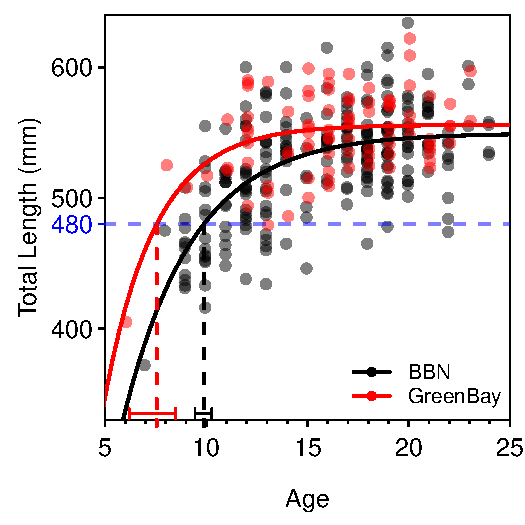
\includegraphics[width=.45\linewidth]{Figs/unnamed-chunk-17-1} 

}



\end{knitrout}
\end{frame}



%###############################################################################
%###############################################################################
\section{Summary}

\begin{frame}[fragile, t]
\frametitle{Summary}
\vspace{-14pt}
\[\Scale[1.5]{ L_{t} = L_{r} + \left(L_{\infty}-L_{r}\right)\left(1-e^{-K(t-t_{r})}\right) }\]
\bigskip
\begin{itemize}
  \item A simple modification of the VBGF allows direct estimation of a parameter of interest, $t_{r}$.
  \begin{itemize}
    \item Same estimates of $L_{\infty}$ and $K$ as with the traditional VBGF.
    \item Same predicted mean lengths-at-age as with the traditional VBGF.
  \end{itemize}
  \pause
  \bigskip
  \item Benefits
  \begin{itemize}
    \item Easy interval estimates of $t_{r}$.
    \item Compare $t_{r}$ between groups with standard (ANCOVA-like) methods.
  \end{itemize}
  \pause
  \smallskip
  \item Costs
  \begin{itemize}
    \item No direct estimate of $t_{0}$ (in the traditional VBGF).
  \end{itemize}
\end{itemize}
\end{frame}


\begin{frame}[fragile, t]
\frametitle{Recommendation}
\vspace{-14pt}
\[\Scale[1.5]{ L_{t} = L_{r} + \left(L_{\infty}-L_{r}\right)\left(1-e^{-K(t-t_{r})}\right) } \]

\vspace{0.5in}

\centerline{\begin{minipage}{0.65\textwidth}
\LARGE Use this modified VBGF in place of the traditional VBGF.
\end{minipage}}
\end{frame}



%###############################################################################
%###############################################################################
\section*{Acknowledgments}
\begin{frame}[fragile, t]
\frametitle{Acknowledgments}
\begin{itemize}
  \item Matthew Belnap for collection and initial processing of Whitefish data.
  \bigskip
  \item Ben Wegleitner, Zach Kleemann, Andrew Gullickson, and Connie Isermann for help processing Whitefish otoliths.
  \bigskip
  \item David Staples (Minnesota DNR) and Joshua McCormick (Oregon Department of Fisheries \& Wildlife) for comments on modified VBGF.
\end{itemize}
\end{frame}


%###############################################################################
%###############################################################################
\section*{Thanks}
\begin{frame}[plain]
\end{frame}




%###############################################################################
%###############################################################################
\section*{Alternative Explanation}

\begin{frame}[fragile, t]
\frametitle{Revisit $t_{0}$}
  \vspace{-6pt}
  \begin{itemize}
    \item Recall that $t_{0}$ is the x-intercept (value of $X$ when $Y=0$).
  \end{itemize}

\begin{knitrout}\footnotesize
\definecolor{shadecolor}{rgb}{0.969, 0.969, 0.969}\color{fgcolor}

{\centering 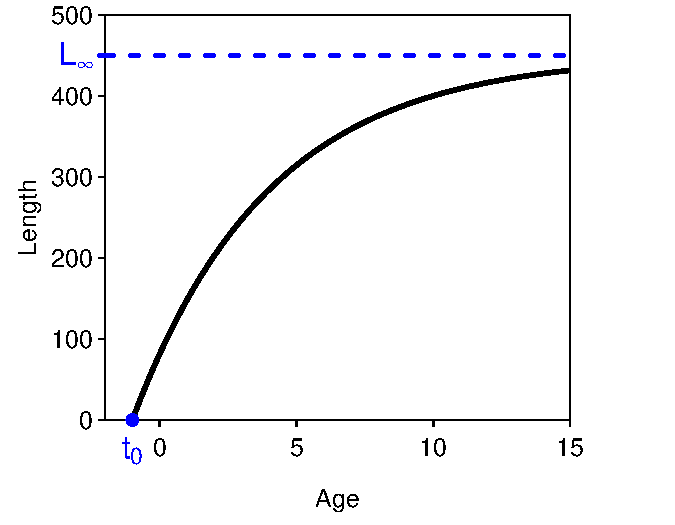
\includegraphics[width=.5\linewidth]{Figs/redefine1-1} 

}



\end{knitrout}
\end{frame}


\begin{frame}[fragile, t]
\frametitle{Revisit $t_{0}$}
  \vspace{-6pt}
  \begin{itemize}
    \item Recall that $t_{0}$ is the x-intercept (value of $X$ when $Y=0$).
  \end{itemize}
\begin{knitrout}\footnotesize
\definecolor{shadecolor}{rgb}{0.969, 0.969, 0.969}\color{fgcolor}

{\centering 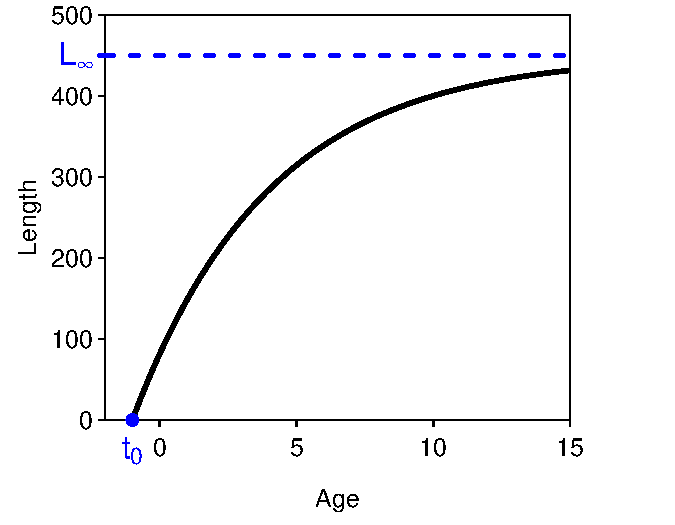
\includegraphics[width=.5\linewidth]{Figs/redefine2-1} 

}



\end{knitrout}
  \begin{itemize}
    \item Let's define $L^{*}_{t}=L_{t}-L_{r}$ (difference in length from critical length).
  \end{itemize}
\end{frame}


\begin{frame}[fragile, t]
\frametitle{Revisit $t_{0}$}
  \vspace{-6pt}
  \begin{itemize}
    \item Recall that $t_{0}$ is the x-intercept (value of $X$ when $Y=0$).
  \end{itemize}
\begin{knitrout}\footnotesize
\definecolor{shadecolor}{rgb}{0.969, 0.969, 0.969}\color{fgcolor}

{\centering 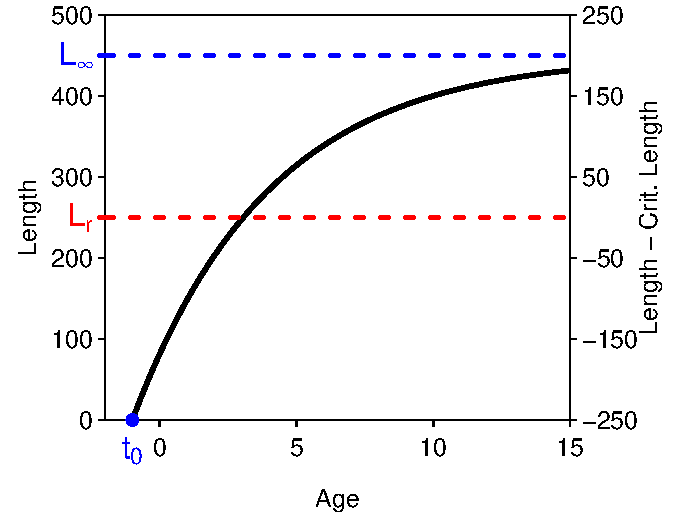
\includegraphics[width=.5\linewidth]{Figs/redefine3-1} 

}



\end{knitrout}
  \begin{itemize}
    \item Let's define $L^{*}_{t}=L_{t}-L_{r}$ (difference in length from critical length).
  \end{itemize}
\end{frame}


\begin{frame}[fragile, t]
\frametitle{Revisit $t_{0}$}
  \vspace{-6pt}
  \begin{itemize}
    \item Recall that $t_{0}$ is the x-intercept (value of $X$ when $Y=0$).
  \end{itemize}
\begin{knitrout}\footnotesize
\definecolor{shadecolor}{rgb}{0.969, 0.969, 0.969}\color{fgcolor}

{\centering 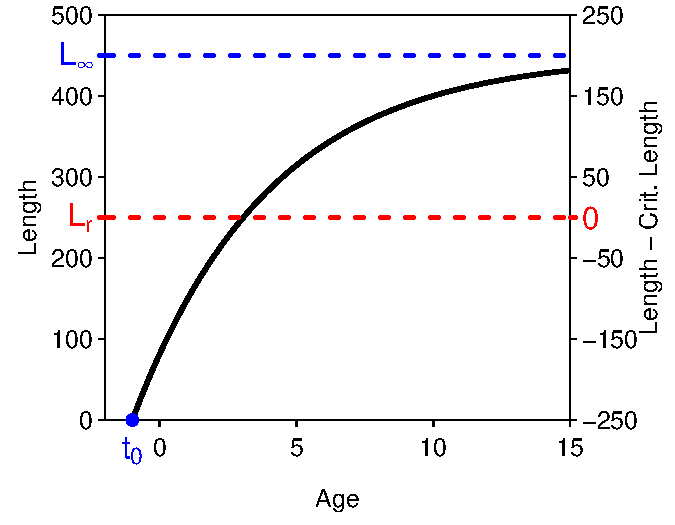
\includegraphics[width=.5\linewidth]{Figs/redefine4-1} 

}



\end{knitrout}
  \begin{itemize}
    \item Let's define $L^{*}_{t}=L_{t}-L_{r}$ (difference in length from critical length).
    \item Thus, $Y=0$ means that $L^{*}_{t}=0$, $L_{t}-L_{r}=0$, and $L_{t}=L_{r}$.
  \end{itemize}
\end{frame}


\begin{frame}[fragile, t]
\frametitle{Revisit $t_{0}$}
  \vspace{-6pt}
  \begin{itemize}
    \item Recall that $t_{0}$ is the x-intercept (value of $X$ when $Y=0$).
  \end{itemize}
\begin{knitrout}\footnotesize
\definecolor{shadecolor}{rgb}{0.969, 0.969, 0.969}\color{fgcolor}

{\centering 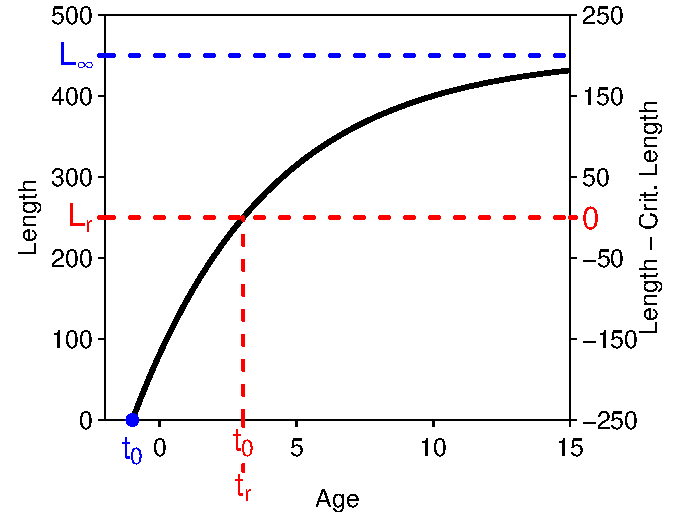
\includegraphics[width=.5\linewidth]{Figs/redefine5-1} 

}



\end{knitrout}
  \begin{itemize}
    \item Let's define $L^{*}_{t}=L_{t}-L_{r}$ (difference in length from critical length).
    \item Thus, $Y=0$ means that $L^{*}_{t}=0$, $L_{t}-L_{r}=0$, and $L_{t}=L_{r}$.
    \item Thus, when using $L^{*}_{t}$, $t_{0} = t_{r}$.
  \end{itemize}
\end{frame}


\begin{frame}[fragile, t]
\frametitle{Modified VBGF}
\begin{itemize}
  \item Therefore, this simple adjustment allows direction estimation of $t_{r}$.
\end{itemize}

\[\Scale[1.5]{ L_{t}-L_{r} = L_{\infty}\left(1-e^{-K(t-t_{r})}\right) }\]

\[\Scale[1.5]{ L_{t} = L_{r} + L_{\infty}\left(1-e^{-K(t-t_{r})}\right) }\]

\end{frame}


\begin{frame}[fragile, t]
\frametitle{Modified VBGF}
\begin{itemize}
  \item However, $L_{\infty}$ is now incorrect.
\end{itemize}

\begin{knitrout}\footnotesize
\definecolor{shadecolor}{rgb}{0.969, 0.969, 0.969}\color{fgcolor}

{\centering 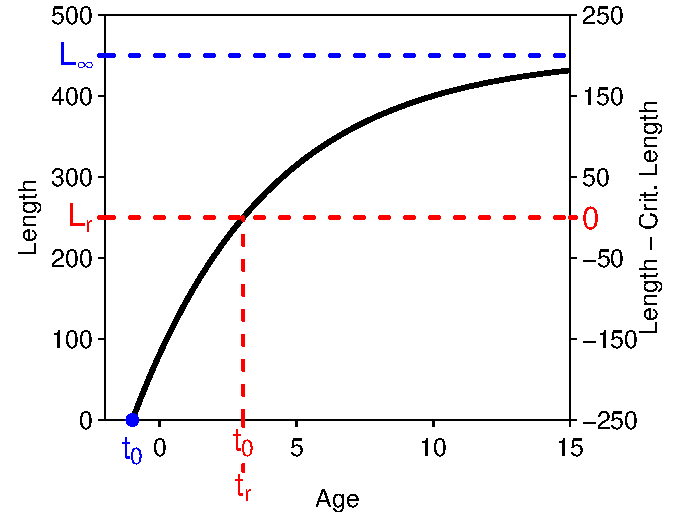
\includegraphics[width=.5\linewidth]{Figs/redefine6-1} 

}



\end{knitrout}
\pause
\begin{itemize}
  \item But this is easily corrected.
\end{itemize}

\[\Scale[1.5]{ L_{t} = L_{r} + \left(L_{\infty}-L_{r}\right)\left(1-e^{-K(t-t_{r})}\right) }\]

\end{frame}

\end{document}
